% Temporal distribution of definitional defects by year of enactment
% TODO: Replace with actual data from pipeline run
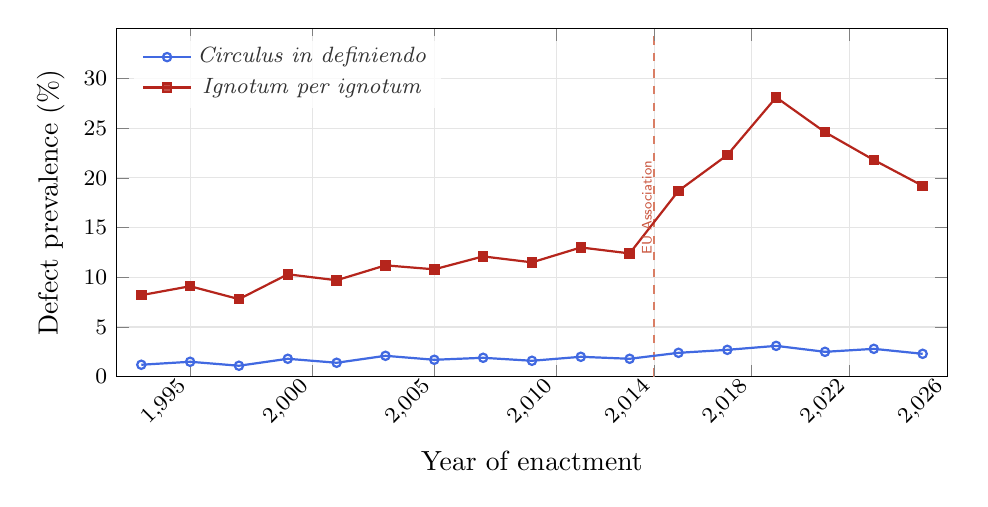
\begin{tikzpicture}
\begin{axis}[
  width=\linewidth,
  height=6cm,
  xlabel={Year of enactment},
  ylabel={Defect prevalence (\%)},
  xmin=1992, xmax=2026,
  ymin=0, ymax=35,
  xtick={1995,2000,2005,2010,2014,2018,2022,2026},
  xticklabel style={font=\footnotesize, rotate=45, anchor=east},
  ytick={0,5,10,15,20,25,30},
  yticklabel style={font=\footnotesize},
  legend style={at={(0.02,0.98)}, anchor=north west, font=\footnotesize, draw=none, fill=white, fill opacity=0.8},
  grid=major,
  grid style={gray!20},
  every axis plot/.append style={thick},
  % Vertical line for Association Agreement
  extra x ticks={2014},
  extra x tick labels={},
  extra x tick style={grid=major, grid style={dashed, BrickRed!50, thick}},
]

% Circulus prevalence (relatively stable)
\addplot[RoyalBlue, mark=o, mark size=1.5pt] coordinates {
  (1993,1.2) (1995,1.5) (1997,1.1) (1999,1.8) (2001,1.4) (2003,2.1)
  (2005,1.7) (2007,1.9) (2009,1.6) (2011,2.0) (2013,1.8)
  (2015,2.4) (2017,2.7) (2019,3.1) (2021,2.5) (2023,2.8) (2025,2.3)
};
\addlegendentry{\emph{Circulus in definiendo}}

% Ignotum prevalence (spikes after 2014)
\addplot[BrickRed, mark=square*, mark size=1.5pt] coordinates {
  (1993,8.2) (1995,9.1) (1997,7.8) (1999,10.3) (2001,9.7) (2003,11.2)
  (2005,10.8) (2007,12.1) (2009,11.5) (2011,13.0) (2013,12.4)
  (2015,18.7) (2017,22.3) (2019,28.1) (2021,24.6) (2023,21.8) (2025,19.2)
};
\addlegendentry{\emph{Ignotum per ignotum}}

% Association Agreement annotation
\node[font=\tiny\sffamily, text=BrickRed!70, rotate=90, anchor=south] at (axis cs:2014.3,17) {EU Association};

\end{axis}
\end{tikzpicture}
